\documentclass[10pt,a4paper]{article}
\usepackage[utf8]{inputenc}
\usepackage[italian]{babel}
\usepackage{amsmath}
\usepackage{amsfonts}
\usepackage{amssymb}
\usepackage{graphicx}
\usepackage{siunitx}
\usepackage[left=2cm,right=2cm,top=2cm,bottom=2cm]{geometry}
\newcommand{\rem}[1]{[\emph{#1}]}
\newcommand{\exn}{\phantom{xxx}}
\usepackage[italian]{babel}
\usepackage[utf8]{inputenc}
\usepackage{siunitx}
\usepackage{graphicx}
\usepackage{xcolor}
\usepackage{amsfonts}
\usepackage{amsmath}
\usepackage{amsthm}
\usepackage{tikz}
\usepackage{pgfplots}
\usepackage{enumitem}
\usepackage{subcaption}
\usepackage{siunitx}
\date{\today}
\usetikzlibrary{shapes.geometric,calc,matrix,arrows,snakes,shapes,patterns}
\title{Esercitazione 11B: Flip-Flop e contatori}
\author{Massimo Bilancioni, Alessandro Foligno, Giuseppe Zanichelli}
\begin{document}	
\maketitle
	
\section{ Flip-Flop D-Latch}
\subsection{Montaggio}
 Si monta il circuito come in Figura \ref{circ}; per attivare a piacimento l'Enable lo si collega con un interruttore a terra in modo tale che quando l'interruttore è aperto, Enable è in alto, quando è chiuso Enable è a terra.
 \begin{figure}[h]
 	\label{circ}
 	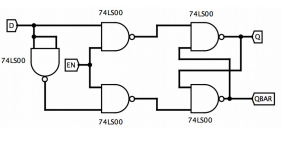
\includegraphics[scale=1]{circuito.png}

 	\caption{schema del circuito realizzato}
 \end{figure}
\subsection{Tempi di ritardo}
Si verifica che quando l'interruttore è aperto ($En=1$), il circuito copia il valore di $D$ su $Q$, nel caso opposto, il valore di $Q$ resta costante. Tenendo il valore di $En$ alto, si manda in ingresso su $D$ un'onda quadra, per misurare il tempo di ritardo. \\Le misure ricavate sono(i segnali osservati sono riportati in Figura \ref{dlatch}):\\ $\Delta t_{salita}\approx40 ns$
\\$\Delta t_{discesa}\approx60 ns$\\
\begin{figure}[h]

	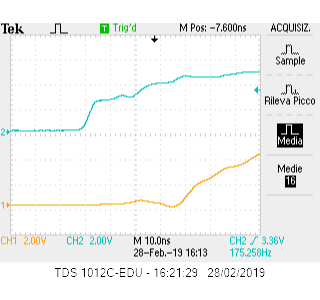
\includegraphics[scale=0.7]{ritardo2.png}
	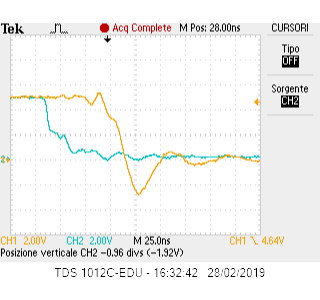
\includegraphics[scale=0.7]{ritardodiscesa2.png}
	\caption{D-Latch con Enable on e in ingresso un'onda quadra: tempo di ritardo in salita e discesa}
		\label{dlatch}
\end{figure} 
La differenza di tempi fra salita e discesa può essere spiegata dando un'occhiata al circuito. Quando $D$ va in alto, il nuovo segnale deve passare attraverso il primo NAND e dare FALSE, dopodichè il NAND successivo restituirà immediatamente TRUE, indipendentemente dal segnale su $\bar{Q}$. Invece, quando $D$ diventa FALSE,il NAND che restituisce $Q$ avrà ad un ingresso TRUE e all'altro $\bar{Q}$, quindi affinchè il segnale su $Q$ sia quello giusto, deve prima arrivare il segnale corretto su $\bar{Q}$ e quindi bisogna passare attraverso altri due NAND, con un ritardo di circa $10 ns$ ciascuno. Questo spiega anche perchè il segnale sull'oscilloscopio(arancione) è così diverso da quello in ingresso (quello blu).

\textcolor{red}{NON SO SE DEVI ANCORA FINIRE IN OGNI CASO AGGIUNGI L'ENABLE LA FIGURA}



\section{ Divisori di frequenza }

Si è montato il circuito e si è verificato il corretto funzionamento del contatore con un impulso a bassa frequenza.



Abbiamo inviato un clock a una frequenza di circa $f\simeq 50 \si{\kilo \hertz}$; nelle immagini che seguono compaiono  rispettivamente $Q0$, $Q1$, $Q2$  (in giallo) sovrapposti al clock (in blu), dalle figure si vede che le frequenze sono effettivamente $1/2$, $1/4$, $1/8$ di $f$. Per $Q3$, segnale di cui non compare l'immagine è stato verificato che la sua frequenza fosse $1/16$ di quella del clock.

\begin{figure}[h]

			\centering

			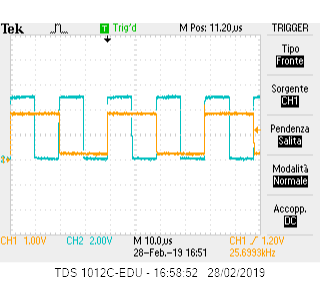
\includegraphics[scale=0.85]{1mezzo}

			\caption{sengale $Q0$ in blu}

			\label{fig:plh}

\end{figure}

\begin{figure}[h]

			\centering

			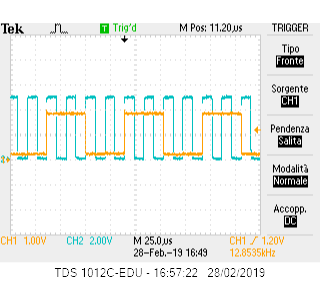
\includegraphics[scale=0.85]{1quarto}

			\caption{sengale $Q1$ in blu}

			\label{fig:plh}

\end{figure}

\begin{figure}[h]

			\centering

			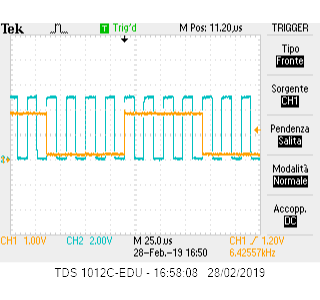
\includegraphics[scale=0.85]{1ottavo}

			\caption{sengale $Q2$ in blu}

			\label{fig:plh}

\end{figure}

Tramite l'oscilloscopio si è poi misurato il ritardo tra la transizione del clock e quella di $Q0$, $Q1$, $Q2$ e $Q3$; in particolare si è misurato l'intervallo temporale che intercorreva da quando la tensione in ingresso passava per il $50\%$ del valore massimo a quando l'uscita passava per  il $50\%$ del valore massimo. Nelle Figure \ref{fig:t1} e \ref{fig:t2} sono mostrati il segnale di clock (in blu) e $Q0$ (in giallo) rispettivamente quando il segnale  $Q0$ passa da alto a basso e da basso ad alto. I ritardi misurati per questa uscita 

sono nel primo caso $t\ped{discesa} = (150 \pm 5)\si{\nano\second}$ e nel secondo  $t\ped{salita} = (30 \pm 5)\si{\nano\second}$.\textcolor{red}{NEL PRIMO PUNTO NON HAI MESSO GLI ERRORI SUI RITARDI, PUOI ANCHE TOGLIERLI QUA MA UNIFORMALI}

Per gli altri tre i ritardi sono gli stessi di $Q0$  nei due casi, infatti le quattro uscite sono quasi perfettamente sincrone tra loro; come esempio  di questa sincronia mostriamo  i segnali $Q0$ e $Q1$ nella transizione da alto a basso in Figura \ref{fig:q0q1}.

Sul datasheet è riportato come tempo di propagazione massimo dal clock all'output (una qualsiasi delle $Q$) $t\ped{max} = 15\si{\nano\second}$ sia per la transizione $HL$ che $LH$. La discrepanza può essere dovuta al tempo di salita del generatore (clock) che avviene in un tempo di circa $50 \si{\nano\second}$, questo potrebbe giustificare il risultato ottenuto per $t\ped{salita} $ tuttavia non giustifica l'asimmetria dei due risultati e il valore misurato per $t\ped{discesa}$.



\begin{figure}[h]

			\centering

			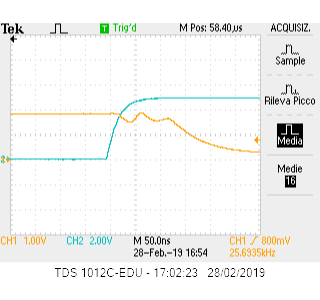
\includegraphics[scale=0.85]{tcounter}

			\caption{ritardo di $Q0$ nel passare da alto a basso}

			\label{fig:t1}

\end{figure}

\begin{figure}[h]

			\centering

			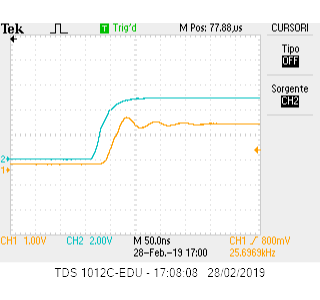
\includegraphics[scale=0.85]{tcounter_1}

			\caption{ritardo di $Q0$ nel passare da basso ad alto}

			\label{fig:t2}

\end{figure}



\begin{figure}[h]

			\centering

			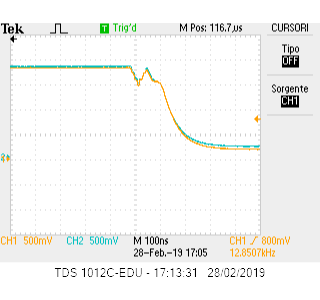
\includegraphics[scale=0.85]{Q0Q1sincroni}

			\caption{quasi perfetta sincronia tra i segnali $Q0$ e $Q1$ quando entrambi diventano bassi}

			\label{fig:q0q1}

\end{figure}





Per resettare il circuito a $10$  abbiamo collegato i segnali $Q1$ e $Q3$ a una porta NAND e l'uscita della porta,  al $\overline{\mathrm{CLR}}$ del contatore di modo che appena entrmabi fossero stati alti il conteggio si sarebbe resettato. 

In Figura \ref{fig:dec} compare il segnale $Q1$ in giallo  e il segnale $Q3$ in blu, quando diventano entrambi alti, cioè quando il contatore è a 10 si vede che dopo un tempo pari al periodo del clock si resetta e  i due segnali diventano bassi. Se osservo l'uscita del NAND questa è bassa per un periodo del clock ogni 11 e quindi ha frequenza 1/11 di CLK. Per ottenere la frequenza di 1/10 come rischiesto dal testo avremmo dovuto resettare il contatore a 9 usando come ingressi del NAND $Q0$ e $Q3$.
\begin{figure}[h]
	\centering
	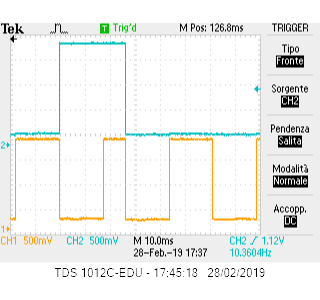
\includegraphics[scale=0.85]{decadico.png}
	\caption{contatore che si resetta arrivato a 10}            
	\label{fig:dec}                    
\end{figure}

\section{Shift register con D-Latch}
\subsection{Montaggio e funzionamento}
Il circuito è stato montato come in figura. I pin CLR sono stati collegati tramite una resistenza di pull-up ai 5V. Il pulsante è stato usato come un deviatore, in modo da riferire anche i preset.
\begin{figure}[h]
	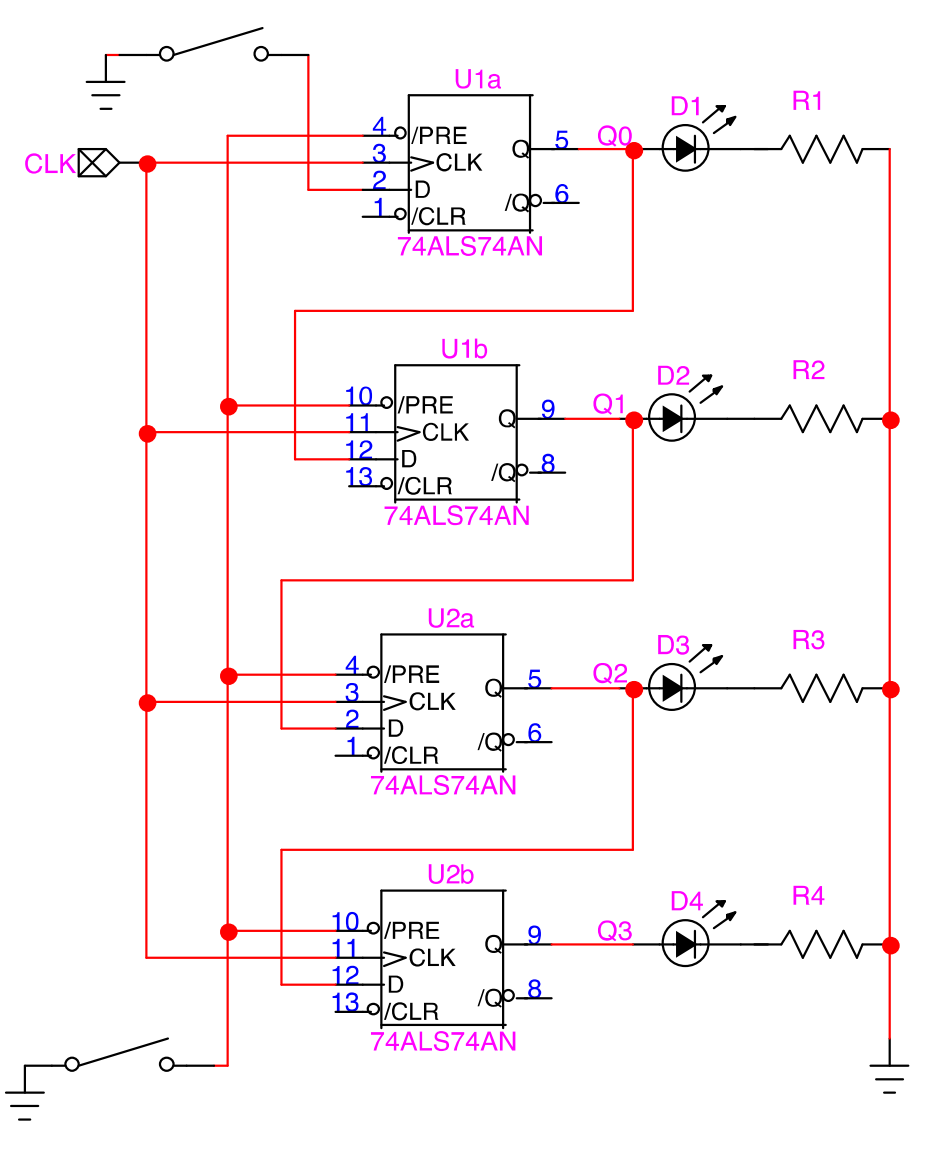
\includegraphics[scale=1]{circuito3.png}
	\caption{Shiftregister} 
	\label{fig:9}                               
\end{figure}
Di default i led sono tutti accesi, se a un dato istante non lo sono  premendo il pulsante di preset si riaccendono tutti (il pin è negato). Il circuito funziona nel seguente modo, ad ogni colpo di clock gli stati dei led in quell'istante  scorrono di uno verso il basso (con riferimento alla figura \ref{fig:9}); lo stato che si inserisce di volta in volta nel primo led, dipende da come è posizionato l'interruttore DIP SWITCH, se ad esempio questo è basso e abbiamo appena premuto il pulsante di preset    i led si spengono in sequenza, partendo dal primo e scorrendo fino all'ultimo con lo spegnimento di uno sfasato di un periodo di clock rispetto allo spegnimento del successivo. 

\subsection{Feedback negato}
Collegando l'uscita negata Q3 all'input del primo FF il circuito inizia a oscillare con una frequenza pari a un ottavo di quella di clock. I led si accendono in successione da Q0 a Q3 per poi spegnersi nello stesso ordine

\begin{figure}[h]
	\centering
	\begin{subfigure}[b]{0.4\linewidth}
		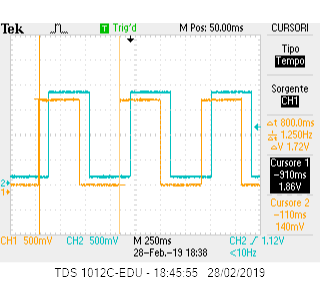
\includegraphics[width=\linewidth]{q0q1periodosr.png}
		\caption{Confronto tra Q0 e Q1, visibile più di un periodo}
	\end{subfigure}
	\begin{subfigure}[b]{0.4\linewidth}
		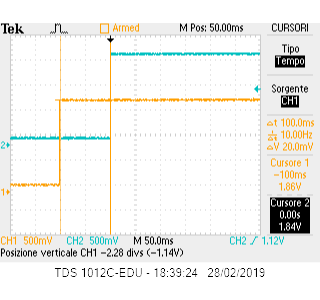
\includegraphics[width=\linewidth]{q0q1sr.png}
		\caption{Confronto tra Q0 e Q1, sfasamento alla salita}
	\end{subfigure}
	\newline
	\begin{subfigure}[b]{0.4\linewidth}
		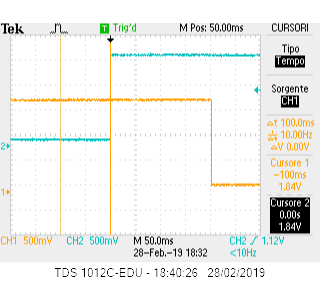
\includegraphics[width=\linewidth]{q0q2sr.png}
		\caption{Q0 e Q2, sfasamento alla salita}
	\end{subfigure}
	\begin{subfigure}[b]{0.4\linewidth}
		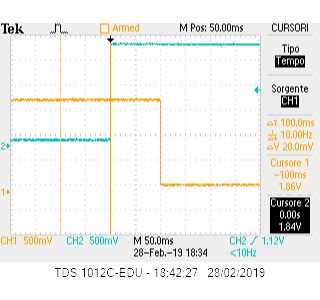
\includegraphics[width=\linewidth]{q0q3sr.png}
		\caption{Q0 e Q3, sfasamento alla salita}
	\end{subfigure}
	\caption{Shift register con feedback negato Q0 nelle quattro immagini è il segnale blu mentre in giallo compaiono Q1,Q2,Q3}
\end{figure}

Nelle figure si può  vedere un confronto tra le onde quadre emesse su ogni piedino e Q0. Si può osservare  lo sfasamento di 1,2,3 tempi di clock.

\end{document}